
\subsubsection{Projection of CMS search for exotic $\PH\to aa \to 2b 2\tau$}\label{Sec:9.1.3}
\begin{center}
 {\it{ by Cecile Caillol}}
\end{center}

This analysis looks for decays of the Higgs boson to pairs of pseudoscalar bosons in the final state of two
$\tau$ leptons and two $b$ quarks~\cite{Sirunyan:2018pzn}. The $\tau\tau$ pair is reconstructed as $e\mu$, $\mu\tau_h$, or $e\tau_h$, depending on the decay modes of the $\tau$ leptons. The symbol $\tau_h$ denotes a $\tau$ lepton decaying hadronically.
Only one $b$ jet with $p_T>20$ \UGeV is required to be reconstructed and tagged as originating from a $b$ quark
because the $b$ jets originating from the pseudoscalar boson are typically soft.
An improved signal sensitivity is obtained by dividing the events in four different
categories depending on the visible invariant mass of the $\PQb$ jet and the $\tau$ candidates, denoted $m_{b\tau\tau}$.
 The thresholds that define the categories depend on the final state.
The categories with low $m_{b\tau\tau}$ are enriched in signal events, while the categories with large $m_{b\tau\tau}$ help to
constrain the backgrounds. The results are extracted with a maximum likelihood fit of the visible $\Pgt\Pgt$ mass spectrum.
The dominant backgrounds at low $\ma$ are $\ttbar$ production as well as events with jets misidentified as $\Pgt$
candidates, whereas the Drell--Yan background starts to contribute for $m_a>45$ \UGeV values. This analysis
is only sensitive to pseudoscalar masses above 15 \UGeV. The sensitivity of the analysis mostly comes from the low $m_{b\tau\tau}$
category, which is statistically limited, and the statistical uncertainty strongly dominates the results.

The extrapolations summarised in Ref.~\cite{CMS-PAS-FTR-18-035},  and presented in this section and the next two assume that the CMS experiment will have a similar level of detector and triggering performance during the HL-LHC operation as it provided during the LHC Run~2
period~\cite{CMSCollaboration:2015zni, Klein:2017nke, Collaboration:2283187, Collaboration:2293646, Collaboration:2283189}.  
The results of extrapolations, hereafter named projections, are presented for different assumptions on the
size of systematic uncertainties that will be achievable by the time of HL-LHC:
\begin{itemize}
\item {\bf ''Run 2 systematic uncertainties'' scenario:} This scenario assumes that performance of the experimental methods at the HL-LHC will be unchanged with respect to the LHC Run 2 period, and there will be no significant improvement in the theoretical descriptions of relevant physics effects. All experimental and
theoretical systematic uncertainties are assumed to be unchanged with respect to the ones in
the reference Run~2 analyses, and kept constant with integrated luminosity.
\item {\bf ''YR18 systematics uncertainties'' scenario:} This scenario assumes that there will be further
advances in both experimental methods and theoretical descriptions of relevant physics effects.
Theoretical uncertainties are assumed to be reduced by a factor two with respect to the ones in the reference
Run~2 analyses. For experimental systematic uncertainties, it is assumed that those will be reduced by the square root
of the integrated luminosity until they reach a defined lower limit based on estimates of
the achievable accuracy with the upgraded detector.
\end{itemize}

In these scenarios, all the uncertainties related to the limited number of simulated events are neglected,
 under the assumption that sufficiently large simulation samples will be available by the time the HL-LHC becomes operational.

For all scenarios, the intrinsic statistical uncertainty in the measurement is reduced by a
factor $1/\sqrt{\text{R}_\text{L}}$, where $\text{R}_\text{L}$ is the projection integrated luminosity divided by that of the
reference Run~2 analysis.

Table~\ref{tab:systematics} summarises the Run~2 uncertainties for which a lower limit value is set in
the ''YR18 systematics uncertainties'' scenario. Systematic uncertainties in the identification and isolation efficiencies
for electrons and muons are expected to be reduced to around $0.5\%$. The hadronic $\tau$ lepton ($\tau_{\mathrm{h}}$) performance is assumed to remain similar to the current level and therefore the associated
uncertainties are not reduced in this scenario. The uncertainty in the overall jet energy scale (JES) is expected to
reach around 1\% precision for jets with $\pt > 30 \GeV$, driven primarily by improvements for the
absolute scale and jet flavour calibrations. The missing transverse momentum uncertainty is obtained by propagating the JES uncertainties in its computation, yielding a reduction by up to a half of the Run~2 uncertainty. For the identification of b-tagged jets, the uncertainty in the selection efficiency of b (c) quarks, and in misidentifying a light jet is expected to remain similar to the current level, with only the statistical component reducing with increasing integrated luminosity. The uncertainty in the integrated luminosity of the data sample could be reduced down to 1\% by a better understanding of the calibration and fit models employed in its determination, and making use of the finer granularity and improved electronics of the upgraded detectors.

\begin{table}[hbtp]
\footnotesize
\centering
\caption{The sources of systematic uncertainty for which limiting values are applied in ''YR18 systematics uncertainties'' scenario.
}

\begin{tabular}{@{} l p{3cm} c c @{}}
Source       &   Component         & Run~2 unc.             & Projection minimum unc. \\
\hline
Muon ID   &           & $1$--$2\%$            & $0.5\%$        \\
Electron ID &           & $1$--$2\%$            & $0.5\%$        \\
Photon ID   &           & $0.5$--$2\%$            & $0.25$--$1\%$    \\
Hadronic $\Pgt$ ID &         & $6\%$               & Same as Run~2    \\
Jet energy scale &  Absolute    & $0.5\%$               & $0.1$--$0.2\%$   \\
         &  Relative    & $0.1$--$3\%$            & $0.1$--$0.5\%$   \\
         &  Pileup      & $0$--$2\%$            & Same as Run~2  \\
         &  Method and sample & $0.5$--$5\%$          & No limit     \\
         &  Jet flavour       & $1.5\%$             & $0.75\%$     \\
         &  Time stability      & $0.2\%$             & No limit     \\
Jet energy res.   &     & Varies with $\pt$ and $\eta$      & Half of Run~2   \\
$\ptvecmiss$ scale       &     & Varies with analysis selection        & Half of Run~2   \\
b-Tagging   & b-/c-jets (syst.)       & Varies with $\pt$ and $\eta$    & Same as Run~2\\
          & light mis-tag (syst.)   & Varies with $\pt$ and $\eta$       & Same as Run~2      \\
           & b-/c-jets (stat.)    & Varies with $\pt$ and $\eta$       & No limit        \\
          & light mis-tag (stat.)   & Varies with $\pt$ and $\eta$       & No limit           \\
Integrated lumi.    &         & $2.5\%$                         & $1\%$          \\
\end{tabular}
\label{tab:floors}
\vspace{0.5cm}
\label{tab:systematics}
\end{table}


Upper limits at 95\% CL on $(\sigma(h)/\sigma_{\textrm{SM}}) \mathcal{B}(h \to aa \to 2b2\tau)$ are shown in Fig.~\ref{fig:bbtt_proj} for different integrated luminosities and systematic uncertainty scenarios. In this expression, $\sigma_\textrm{SM}$ denotes the SM production cross section of the Higgs boson, whereas $\sigma(\Ph)$ is the $\Ph$ production cross section.
The limits improve proportionally to the square root of the integrated luminosity,
as the analysis is statistically limited. For an integrated luminosity of 3000\fbinv, the difference between the limits in the  systematic scenarios of Run 2 and YR18 is of the order of 5\%, and the limits become another 5\% better if all systematic uncertainties are neglected.

\begin{figure*}[hbpt]
\centering
        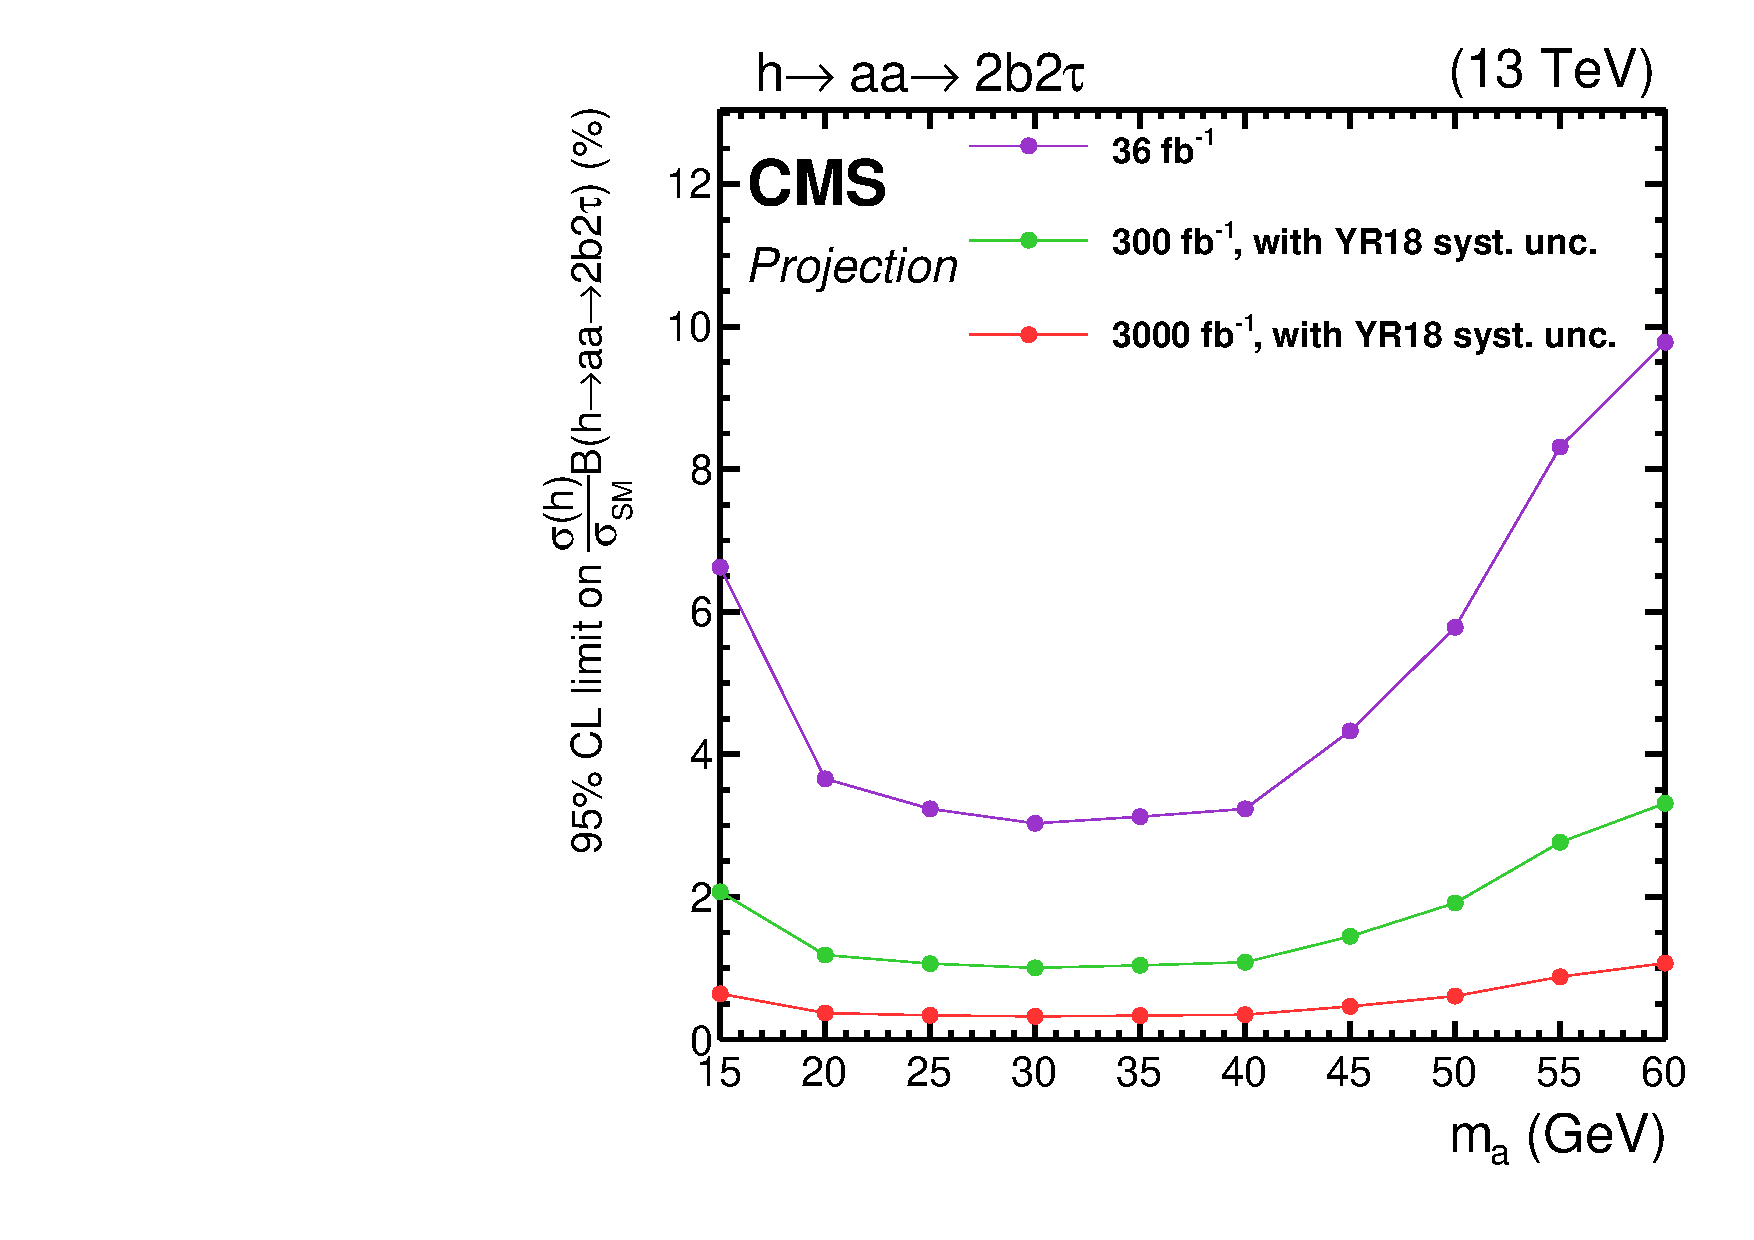
\includegraphics[width=0.49\textwidth]{\main/section9/plots/lim_compare_lum_bbtt.pdf}
        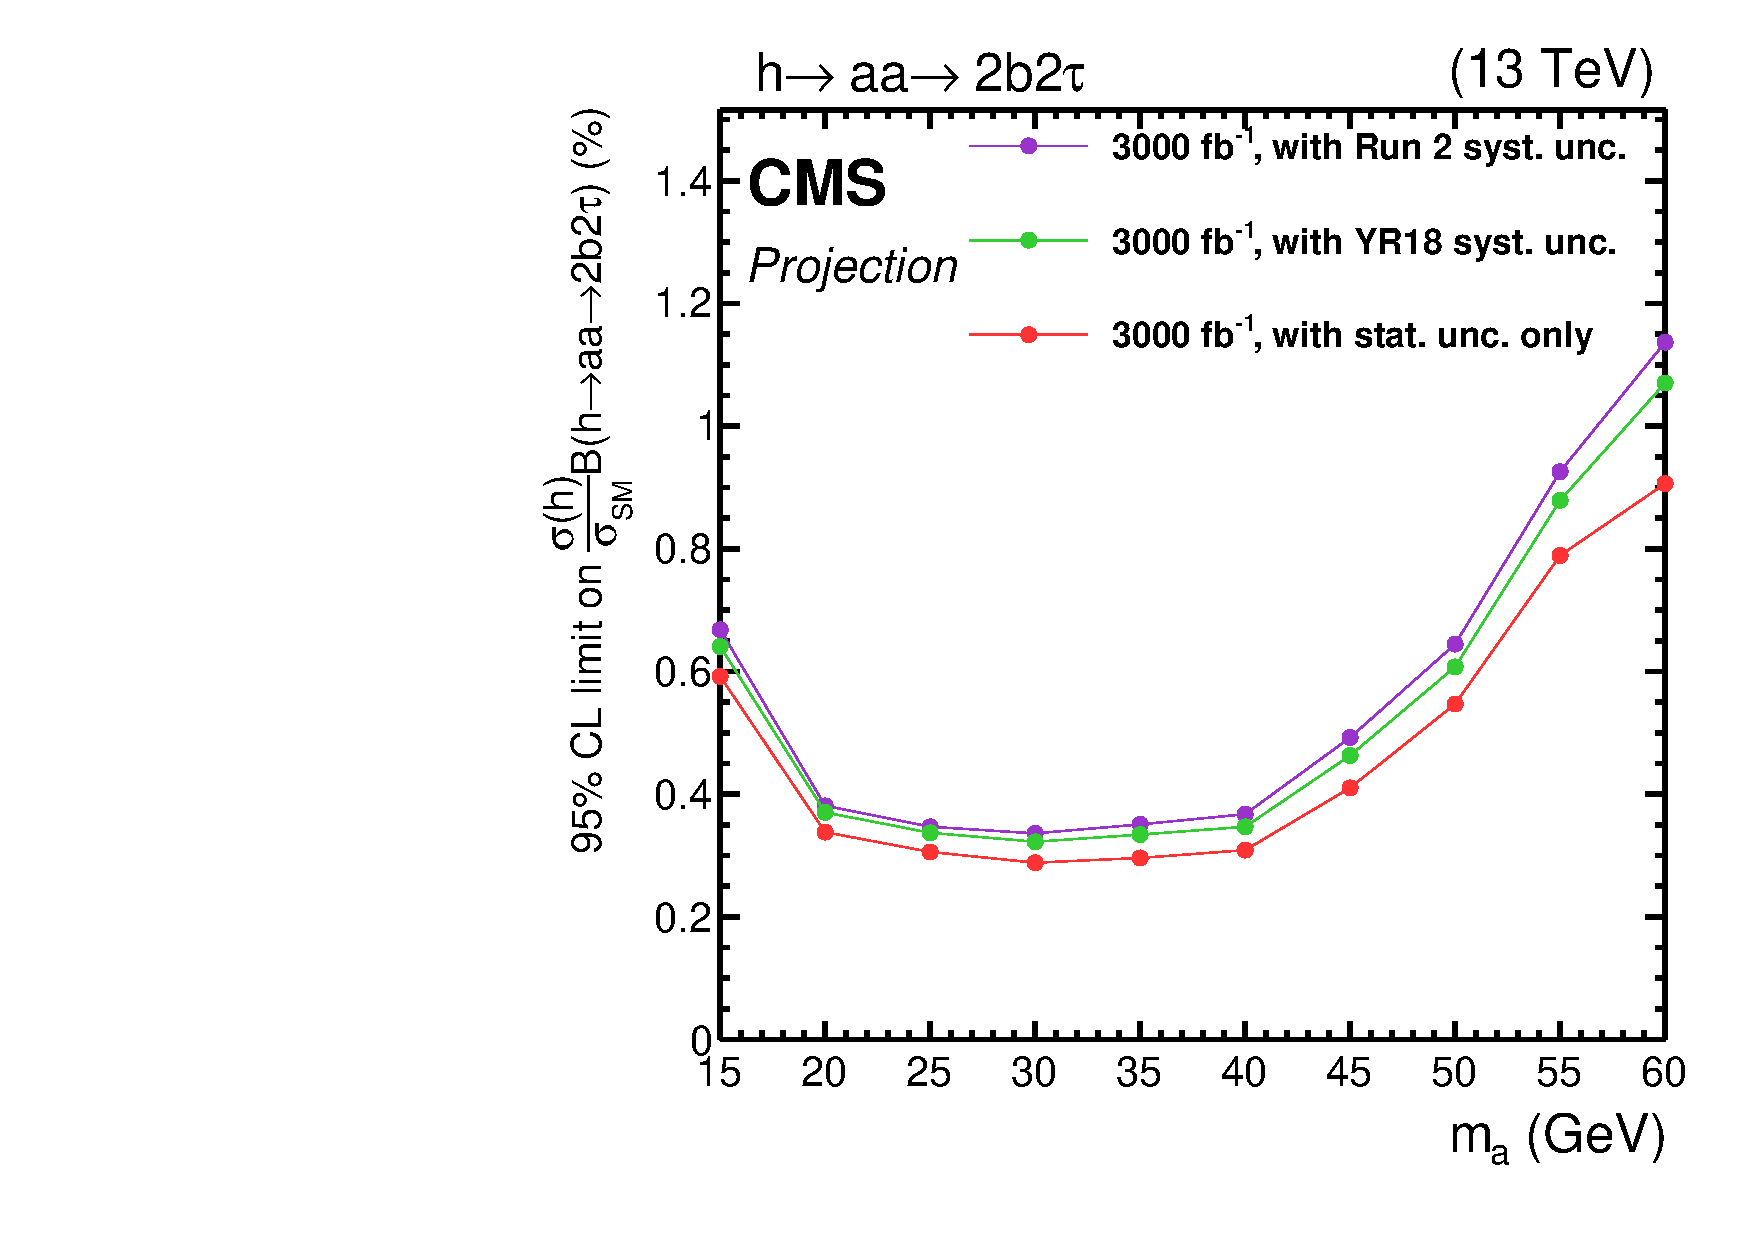
\includegraphics[width=0.49\textwidth]{\main/section9/plots/lim_compare_scenarios3000_bbtt.pdf}\\
    \caption{Left: Projected expected limits on $(\sigma(h)/\sigma_{\textrm{SM}})$ times the branching fraction for $h\to aa\to 2b 2\tau$, for 36, 300, and 3000\fbinv. Right: Projected expected limits $(\sigma(h)/\sigma_{\textrm{SM}}) \mathcal{B}(h\to aa \to 2b2\tau)$, comparing different scenarios for systematic uncertainties for an integrated luminosity of 3000\fbinv.}
    \label{fig:bbtt_proj}
\end{figure*}

The limits of the $h\to aa$ analyses can be converted to limits on $\mathcal{B}(h\to aa)$
in two-Higgs-doublet models extended with
a scalar singlet (2HDM+S)~\cite{PhysRevD.90.075004}, for a given type of model, $m_a$, and $\tan\beta$. The limits in the four types of 2HDM+S are shown
in Fig.~\ref{fig:summary_bbtt}, assuming 3000\fbinv of data with YR18 systematic uncertainties. The colour scale
indicates the upper limits on $(\sigma(h)/\sigma_{\textrm{SM}}) \mathcal{B}(h\to aa)$ that can be set assuming some values for $m_a$ and $\tan\beta$.

\begin{figure*}[hbpt]
\centering
        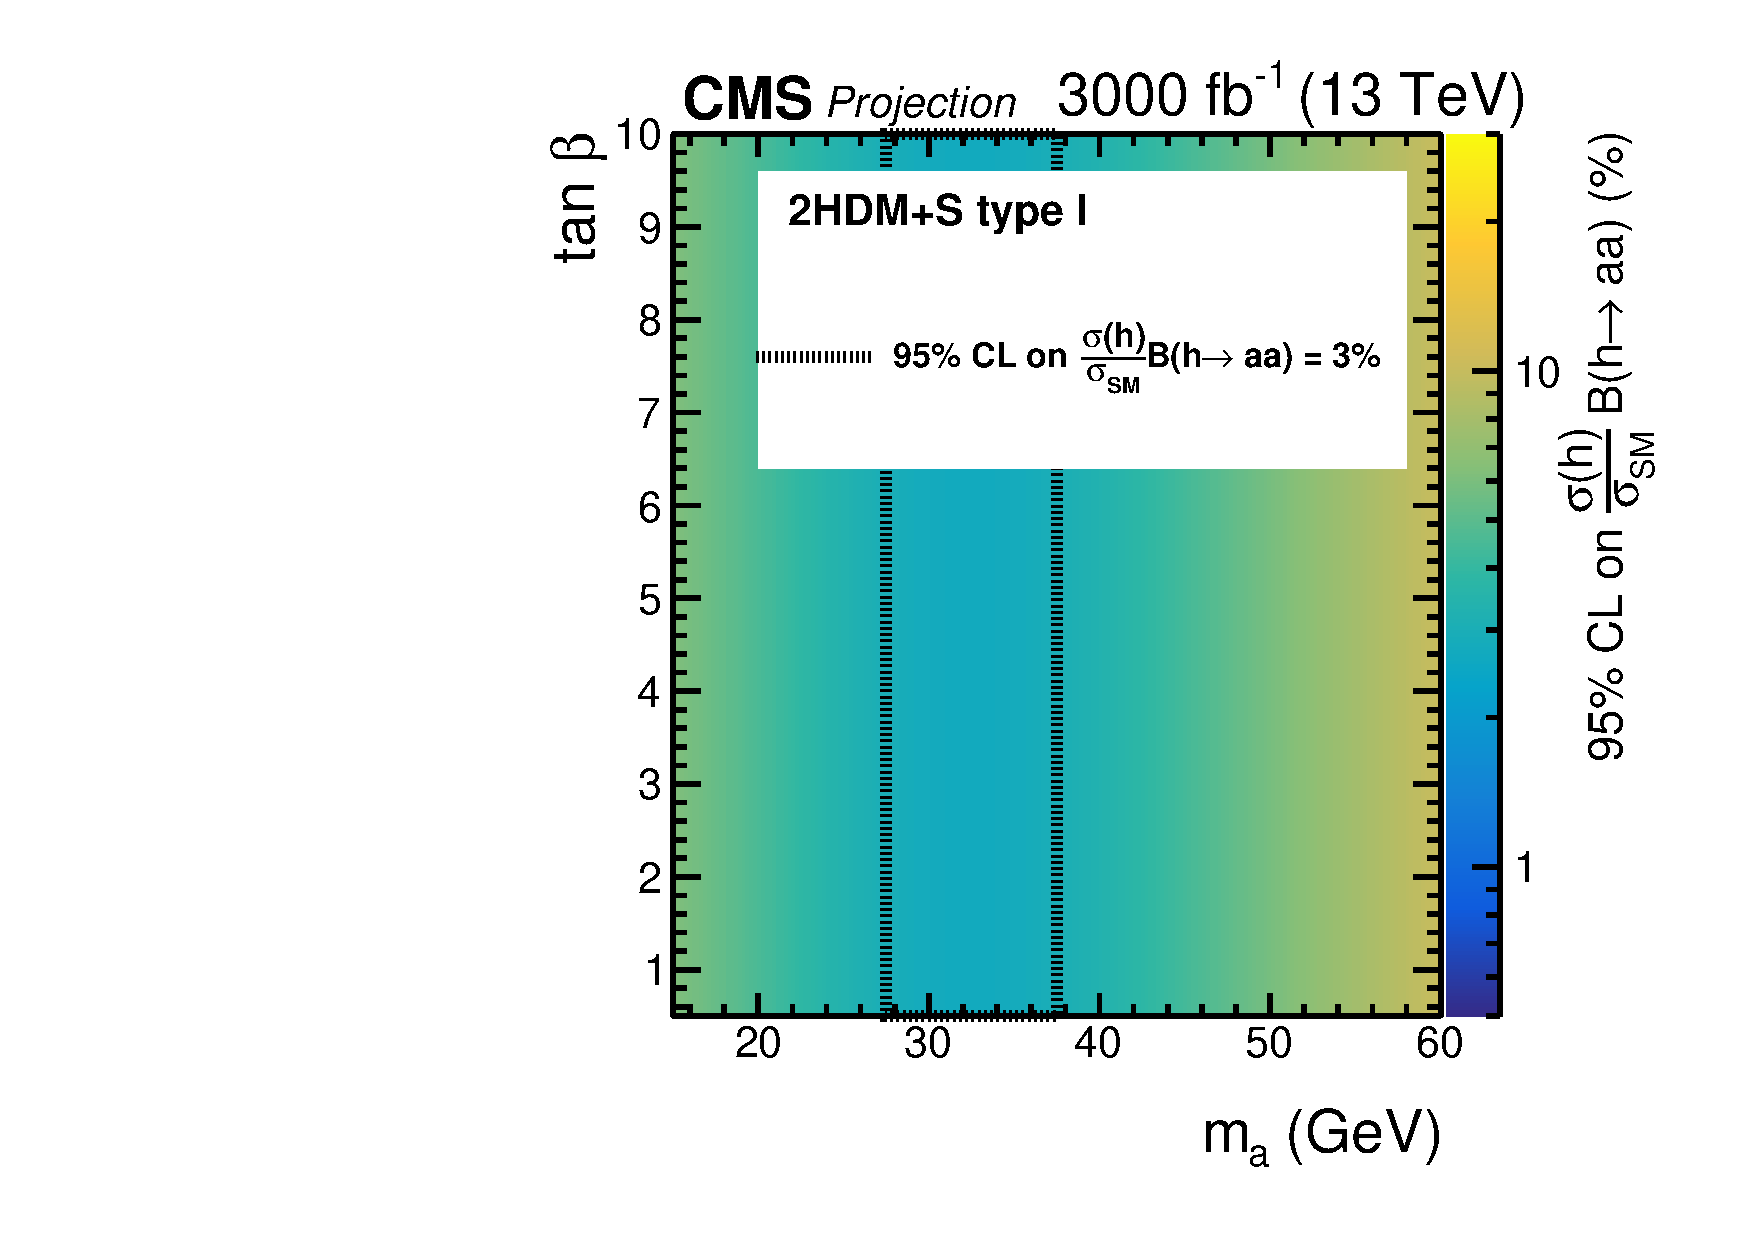
\includegraphics[width=0.49\textwidth]{\main/section9/plots/plot_BRaa_bbttProjection_Type1.pdf}
        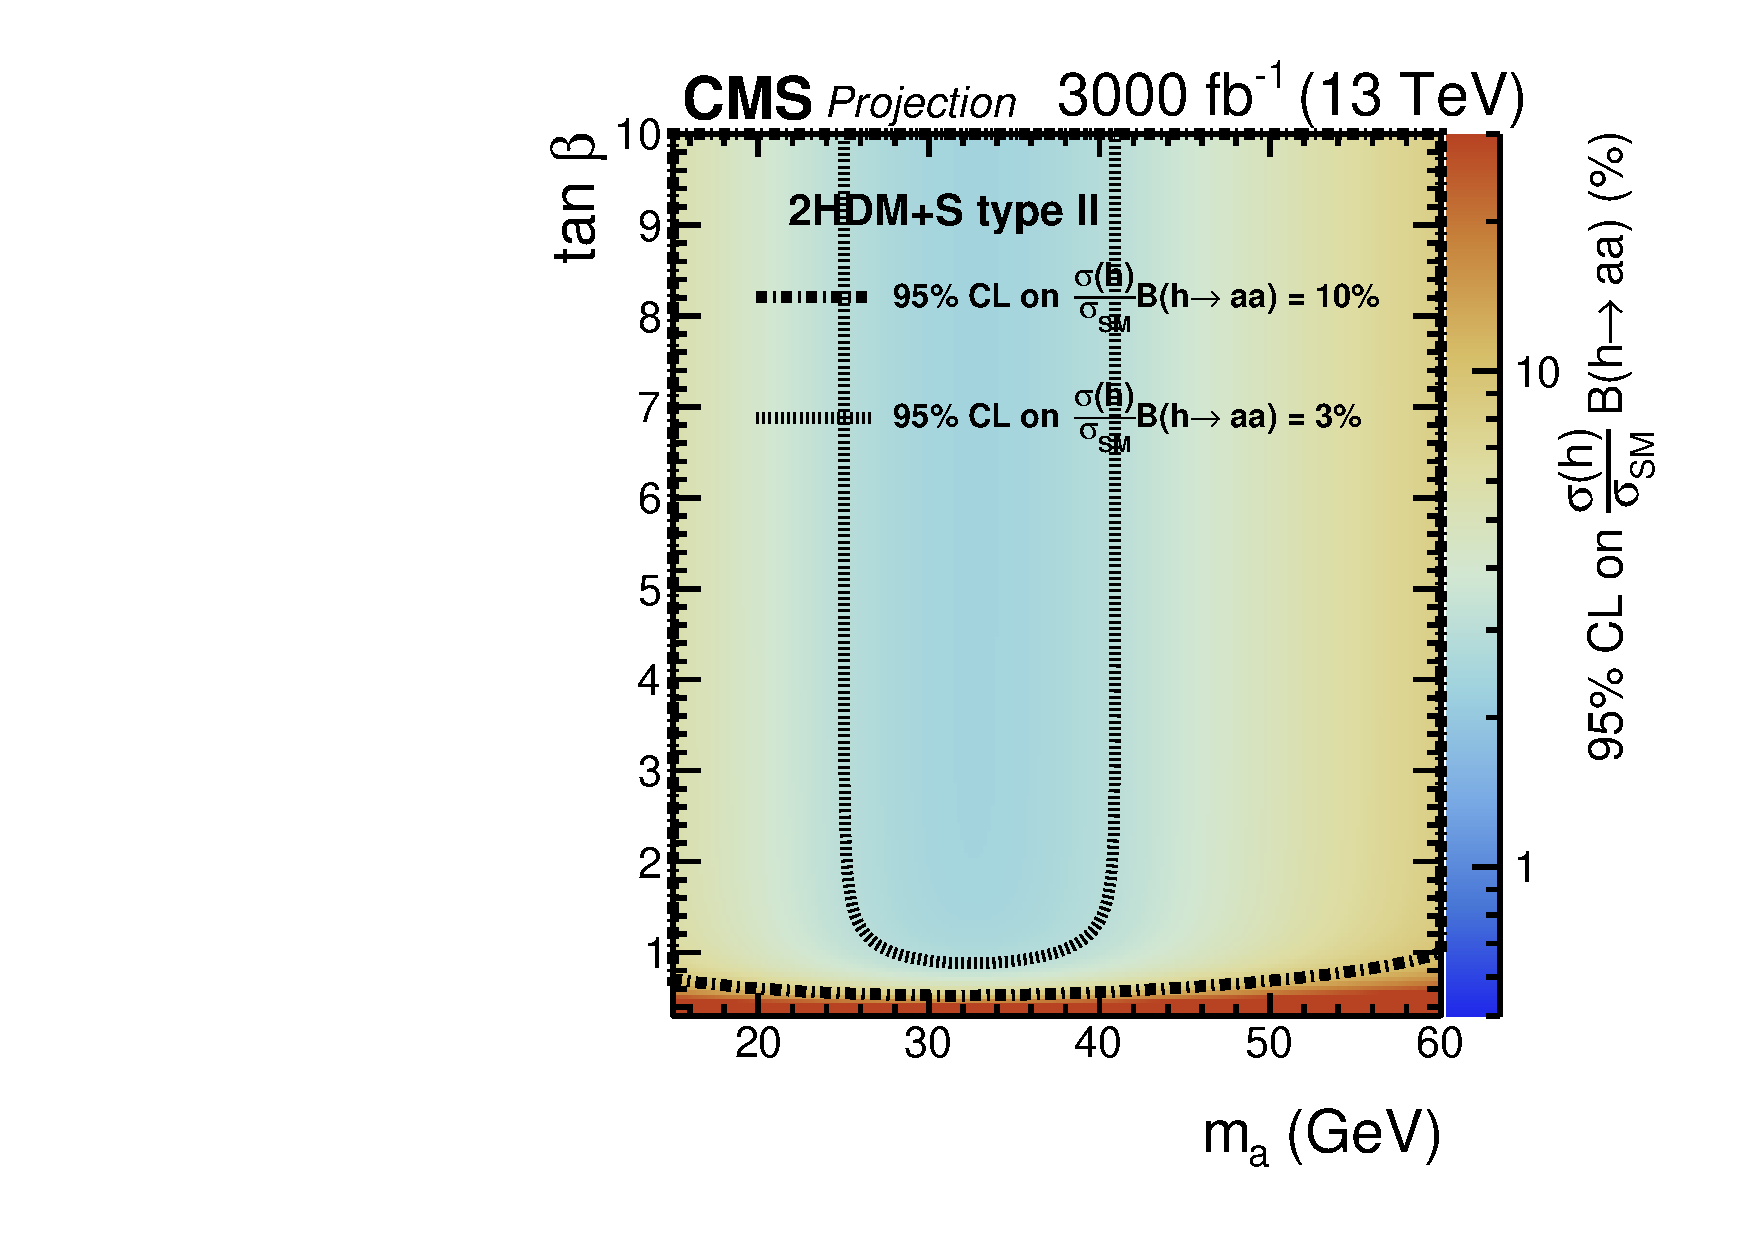
\includegraphics[width=0.49\textwidth]{\main/section9/plots/plot_BRaa_bbttProjection_Type2.pdf} \\
        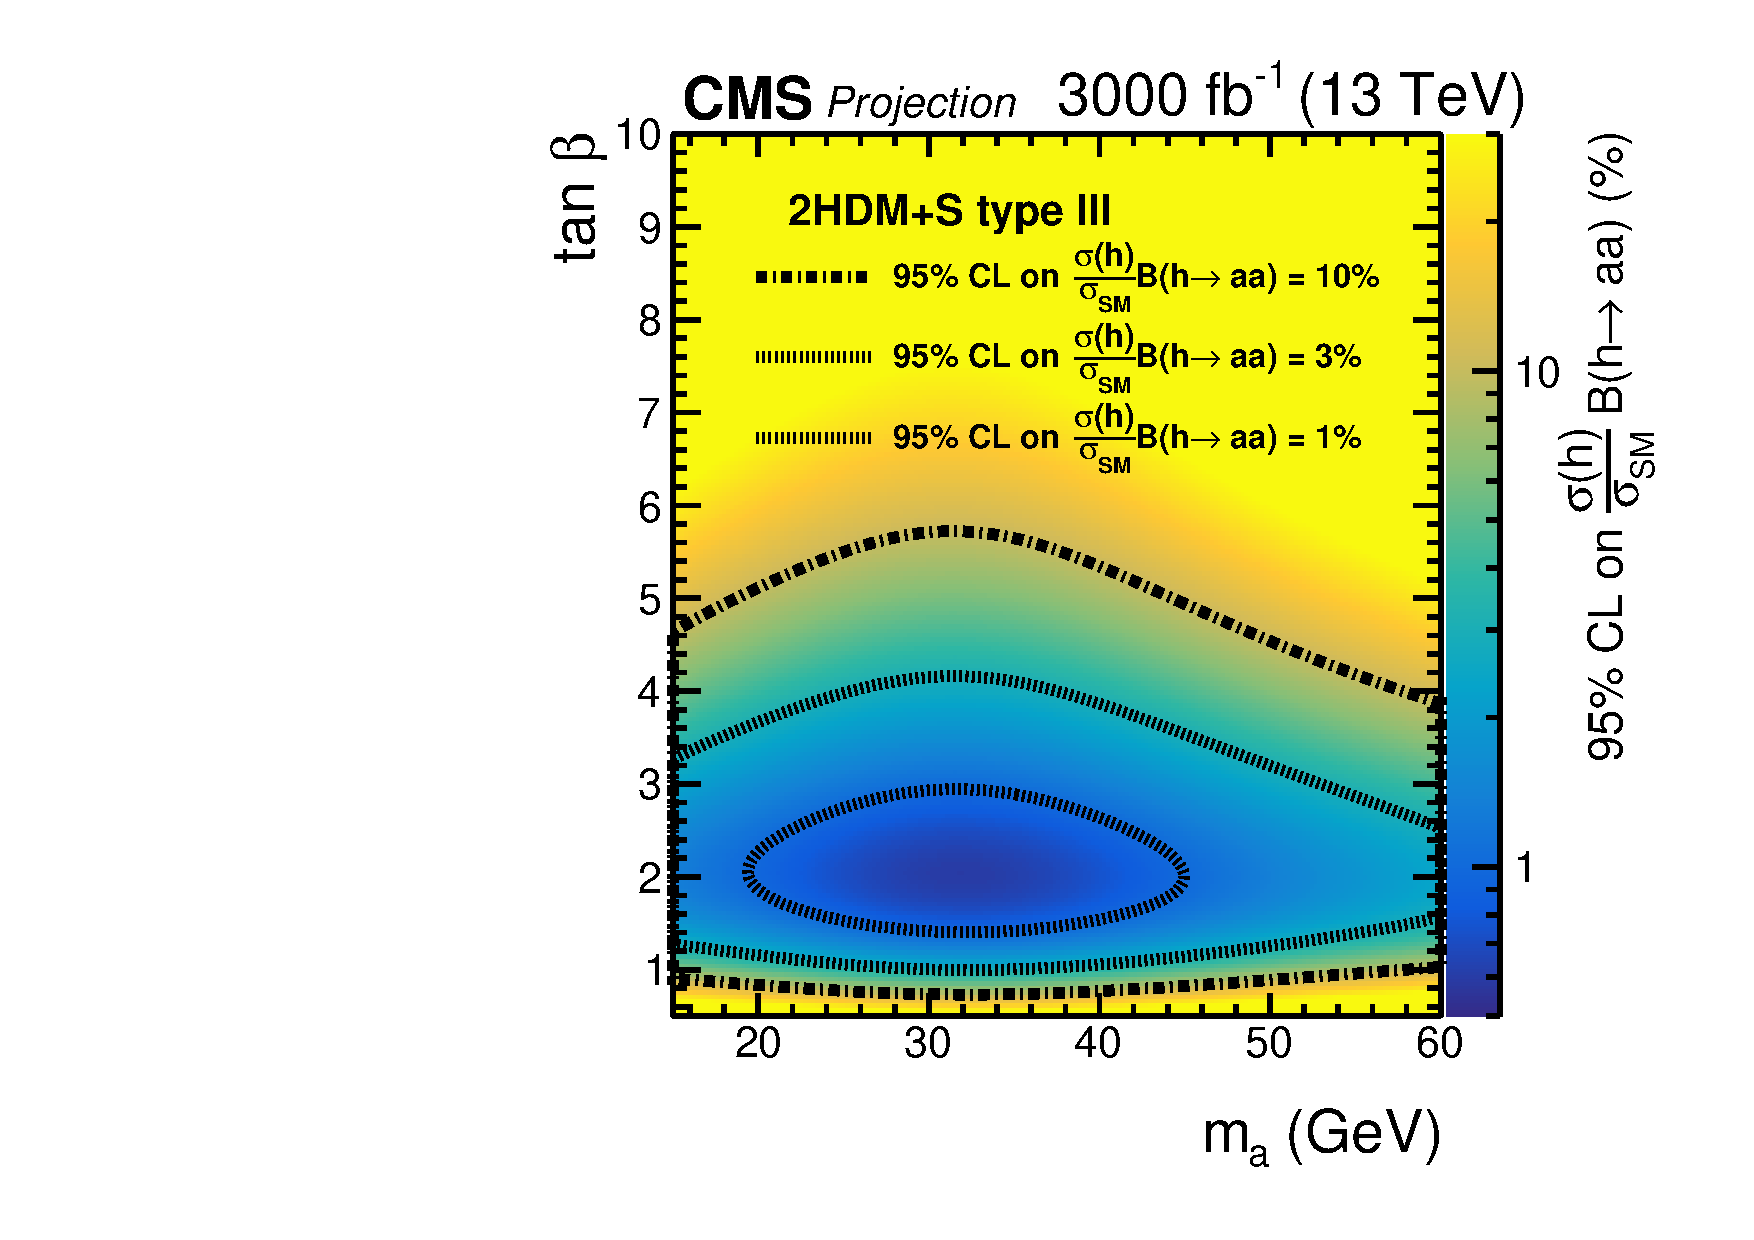
\includegraphics[width=0.49\textwidth]{\main/section9/plots/plot_BRaa_bbttProjection_Type3.pdf}
        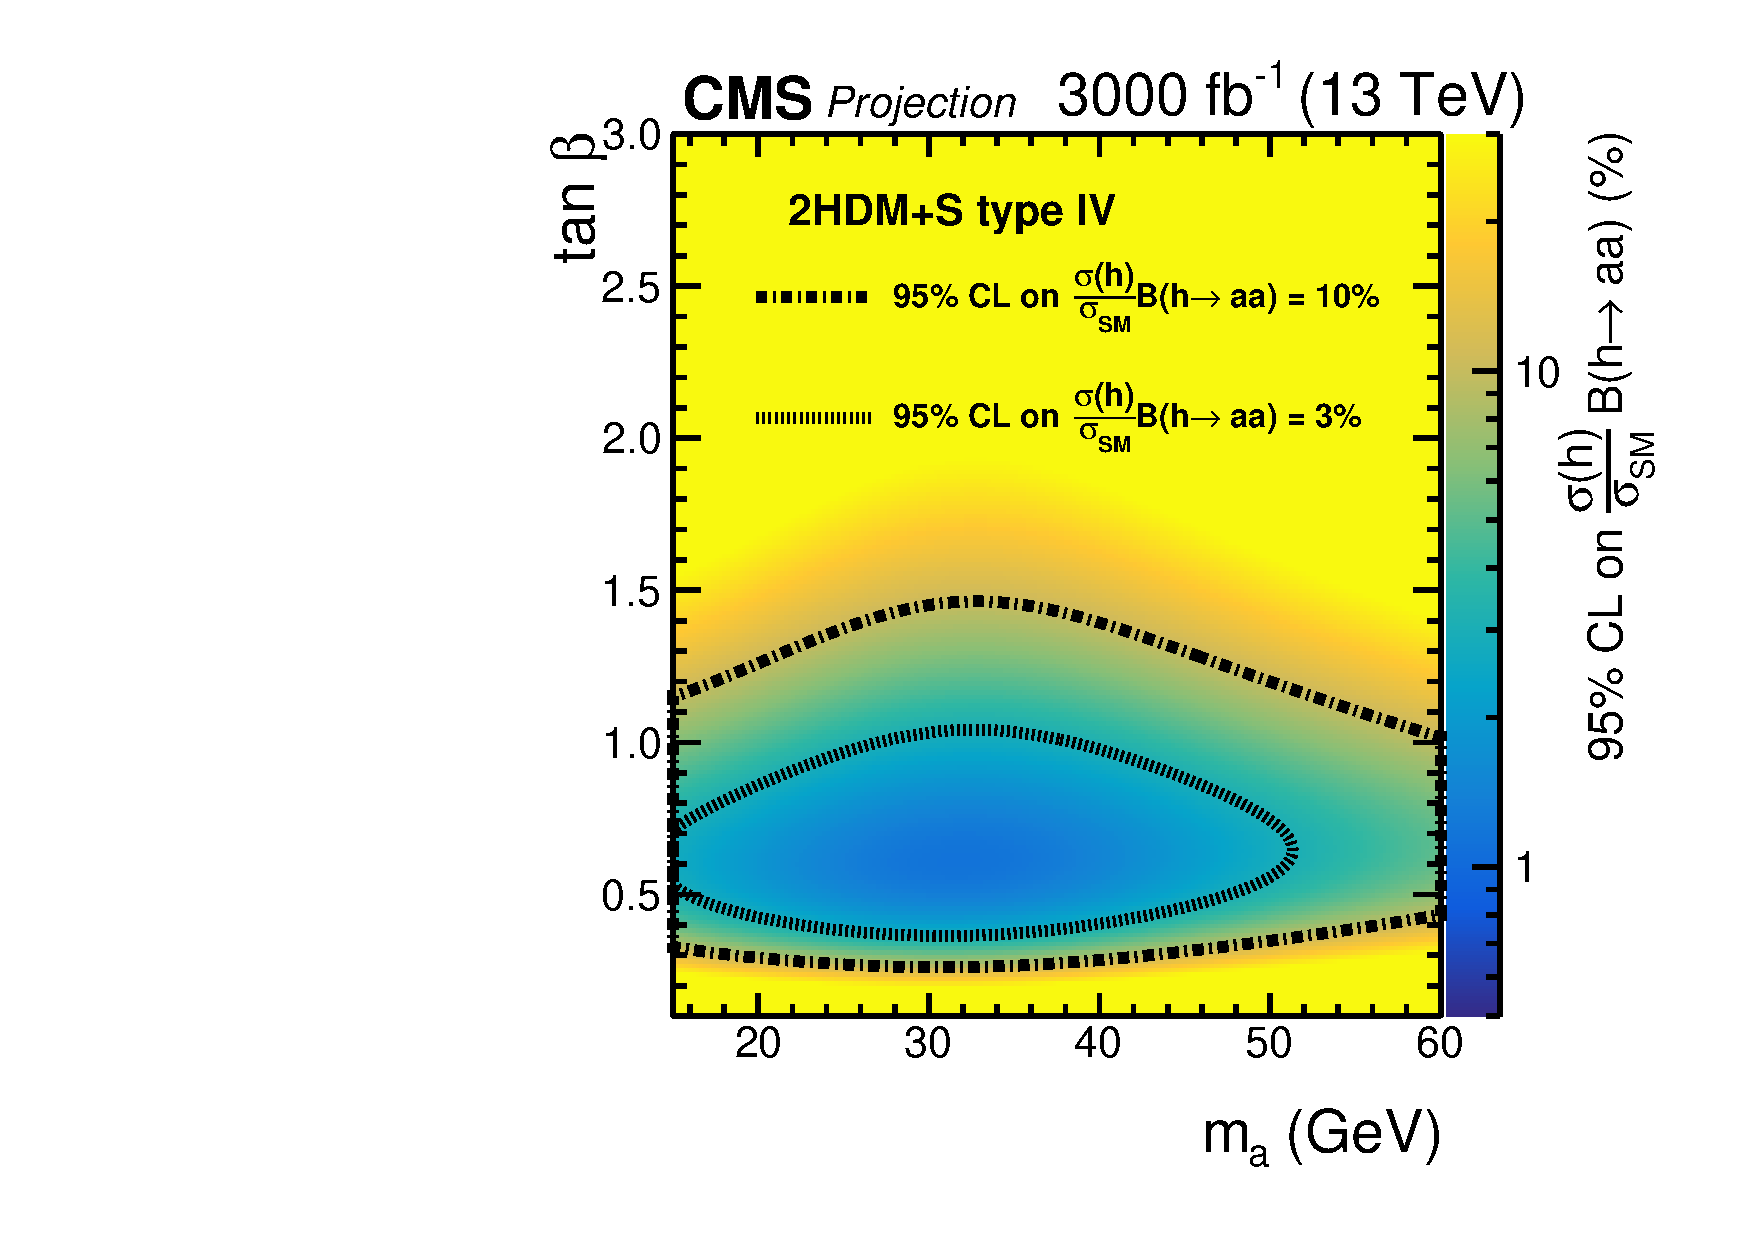
\includegraphics[width=0.49\textwidth]{\main/section9/plots/plot_BRaa_bbttProjection_Type4.pdf}
    \caption{Expected upper limits on $(\sigma(h)/\sigma_{\textrm{SM}}) \mathcal{B}(h\to aa)$ for 3000 fb$^{-1}$ of data with YR18 systematic uncertainties for the $2b 2\tau$ final state in 2HDM+S type-1 (top left), type-2 (top right), type-3 (bottom left), and type-4 (bottom right).}
    \label{fig:summary_bbtt}
\end{figure*}


\subsubsection{Projection of CMS search for exotic $\PH\to aa \to 2\mu 2\tau$}
\begin{center}
 {\it{ by Cecile Caillol}}
\end{center}


This analysis searches for the exotic decay of the Higgs boson to a pair of light pseudoscalars, in the
final state of two muons and two $\tau$ leptons~\cite{Sirunyan:2018mbx}. Pseudoscalar
masses between 15 and 62\GeV are investigated; in this mass range the decay products from the pseudoscalars are
not collimated.
Several $\tau\tau$ pair possibilities are studied in this analysis: $e\mu$, $e\tau_h$,
$\mu\tau_h$, and $\tau_h\tau_h$. In the case where there are 3 muons, the highest-$p_t$ one is paired with
the opposite-sign muon that has the highest-$\pt$ among the other two, while the last muon is considered as
originating from a $\tau$ lepton decay.
To reduce the backgrounds from \PZ\PZ, Z+jets, and \PW\PZ+jets productions, the invariant mass of the muon pair
is required to be above the visible invariant mass of the $\tau\tau$ pair, and the
visible invariant mass of the four objects is required to be less than 110--130 \UGeV depending on the final state.
The limits are extracted with an unbinned maximum likelihood fit of the di-muon mass spectrum.
The backgrounds are characterised by a rather flat di-muon mass spectrum, while the signal $h\to aa \to 2\mu2\tau$
forms a narrow peak in the di-muon mass spectrum.
The number of expected background events below the signal peak is almost zero,
especially at low di-muon mass, and the analysis is strongly statistically dominated.

In the ''YR18 systematics uncertainties'' scenario, in addition to the limiting values detailed in Table \ref{tab:floors}, the uncertainty in the normalisation of the reducible background is not allowed to go lower than 20\% of the value used in Run-2. The corresponding limits for the $h \to aa \to 2\mu2\tau$ search are shown in Fig.~\ref{fig:mmtt_proj}.
They scale approximately inversely with the integrated luminosity at low $m_a$ because the
analysis is close to background-free, while they tend to scale inversely with the square root of the integrated luminosity at higher $m_a$, where the background is more important. This leads to the large improvement at low $m_a$ for 3000\fbinv of collected data shown in Fig.~\ref{fig:mmtt_proj}. The analysis is statistically limited, even with 3000\fbinv of data. The difference between the Run 2 and YR18 systematic uncertainties in terms of upper limits
is up to 5\%, and is the largest at high $m_a$.

\begin{figure*}[hbpt]
\centering
        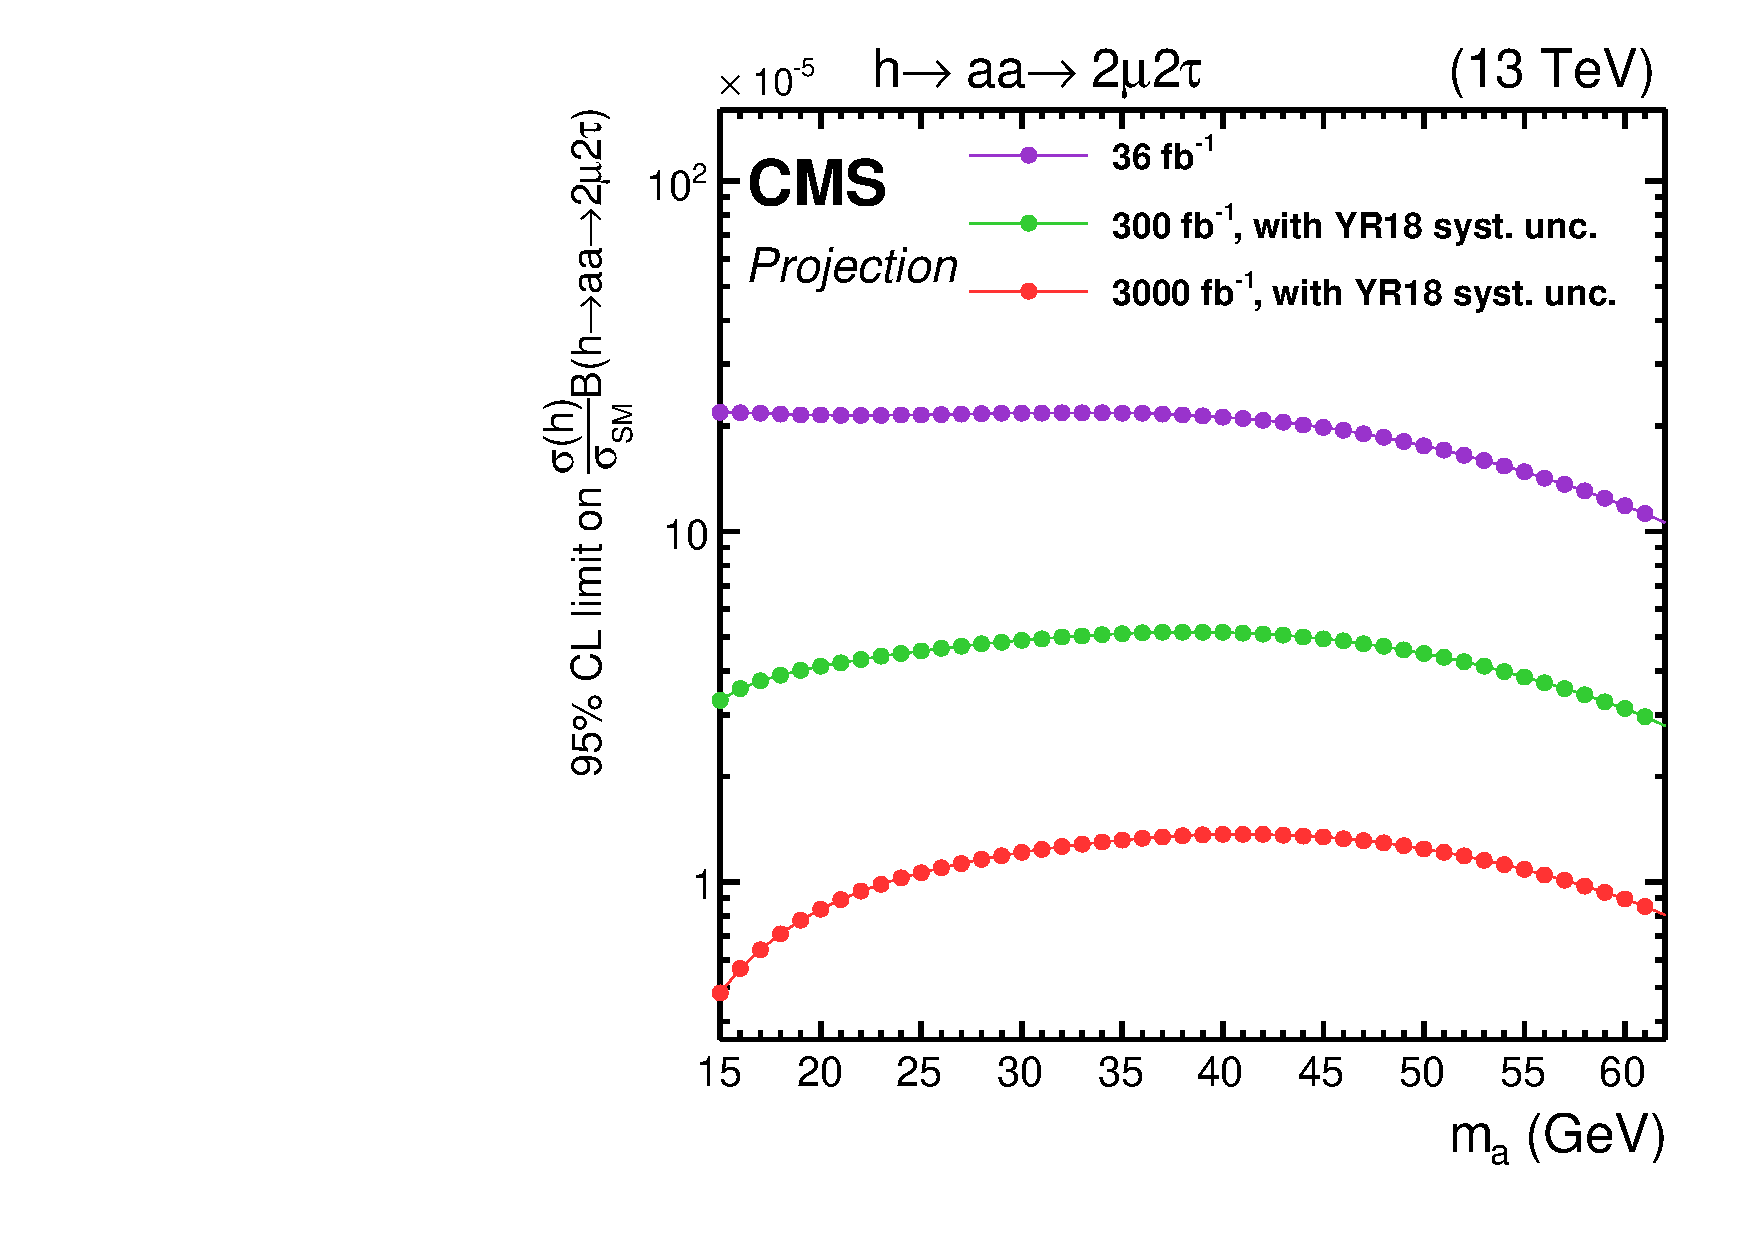
\includegraphics[width=0.49\textwidth]{\main/section9/plots/lim_compare_lum_mmtt.pdf}
        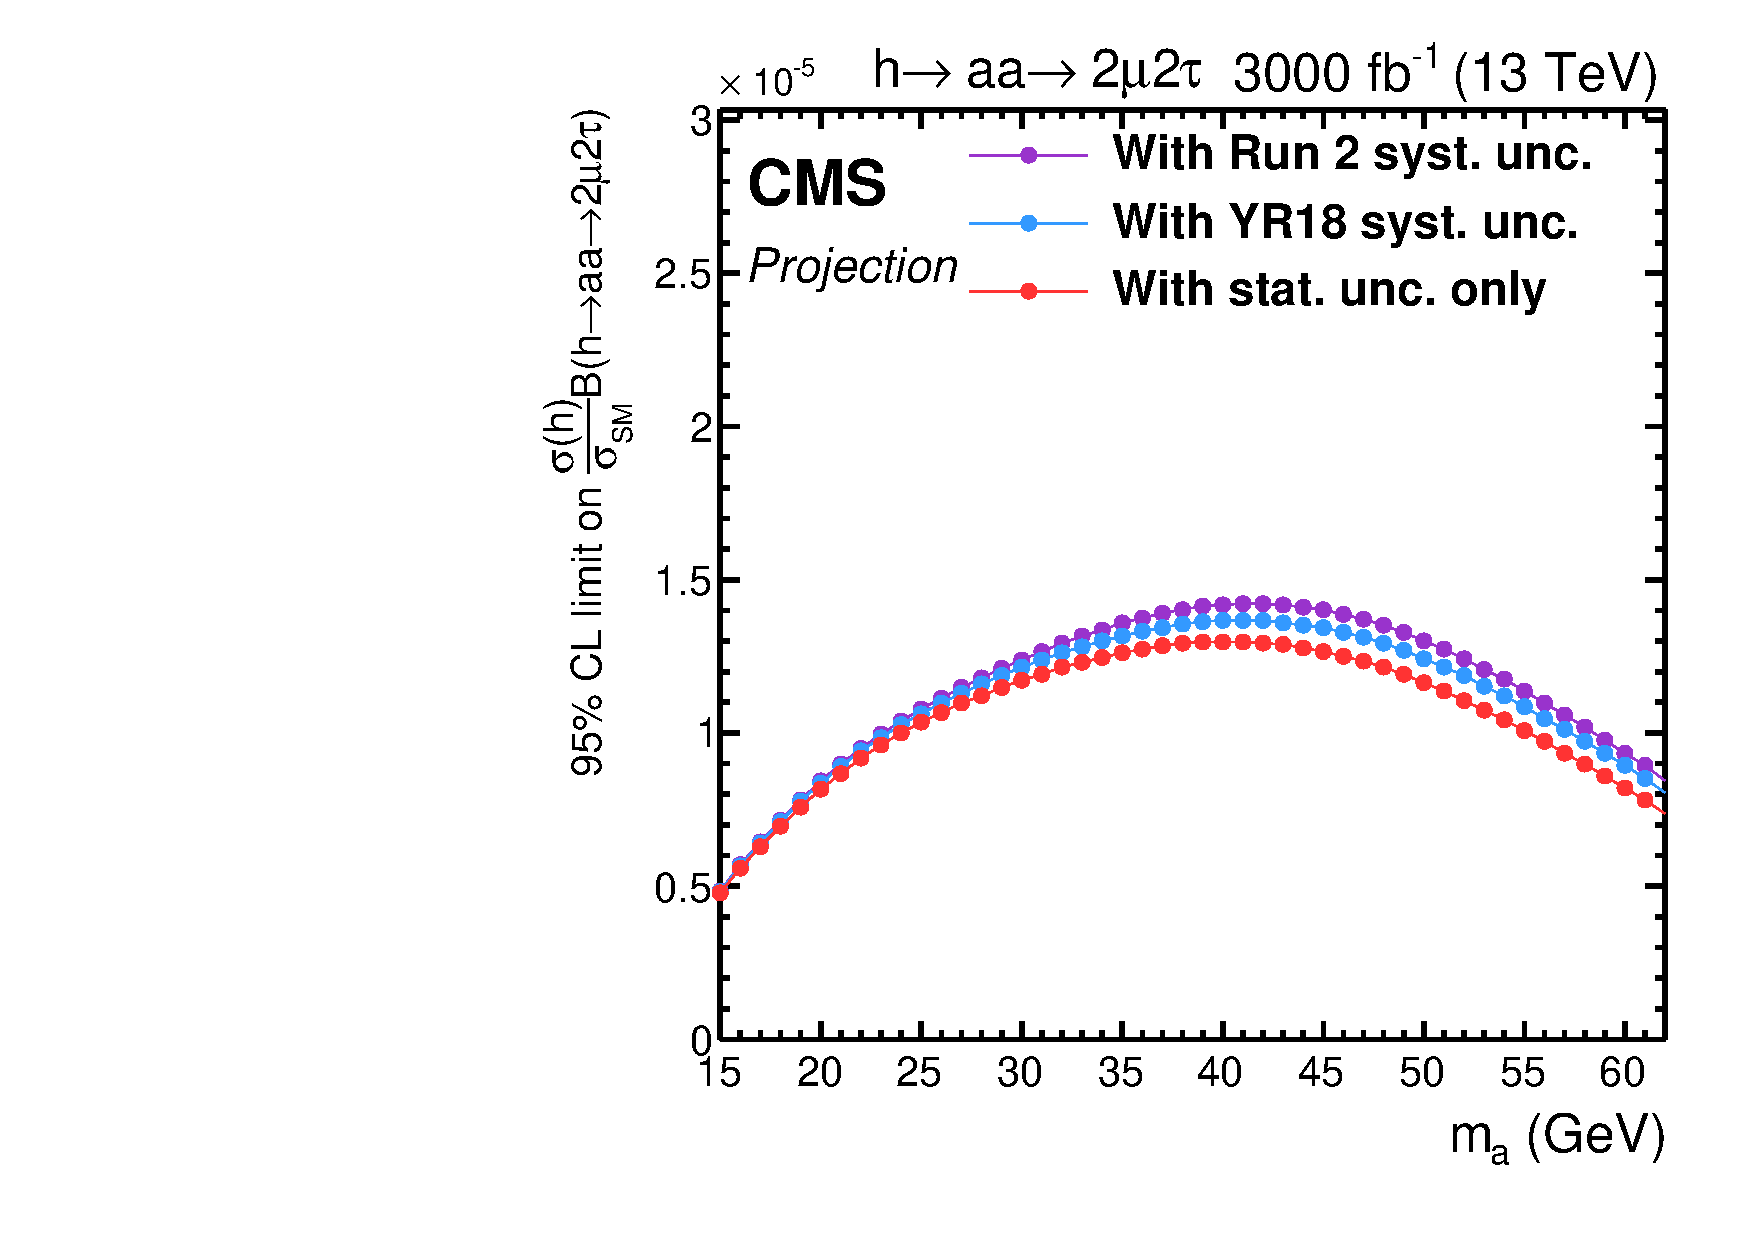
\includegraphics[width=0.49\textwidth]{\main/section9/plots/lim_compare_scenarios3000_mmtt.pdf}\\
    \caption{Left: Projected expected limits on $(\sigma(h)/\sigma_{\textrm{SM}}) \mathcal{B}(h \to aa \to 2\mu 2\tau)$, for 36, 300, and 3000 fb$^{-1}$. Right: Projected expected limits on $(\sigma(h)/\sigma_{\textrm{SM}}) \mathcal{B}(h\to aa \to 2\mu2\tau)$, comparing different scenarios for systematic uncertainties for an integrated luminosity of 3000\fbinv.}
    \label{fig:mmtt_proj}
\end{figure*}

The limits in the four types of 2HDM+S are shown
in Fig~\ref{fig:summary_mmtt} for the $2\mu 2\tau$ analysis, assuming 3000\fbinv of data in the ''YR18 systematics uncertainties'' scenario.

\begin{figure*}[hbpt]
\centering
        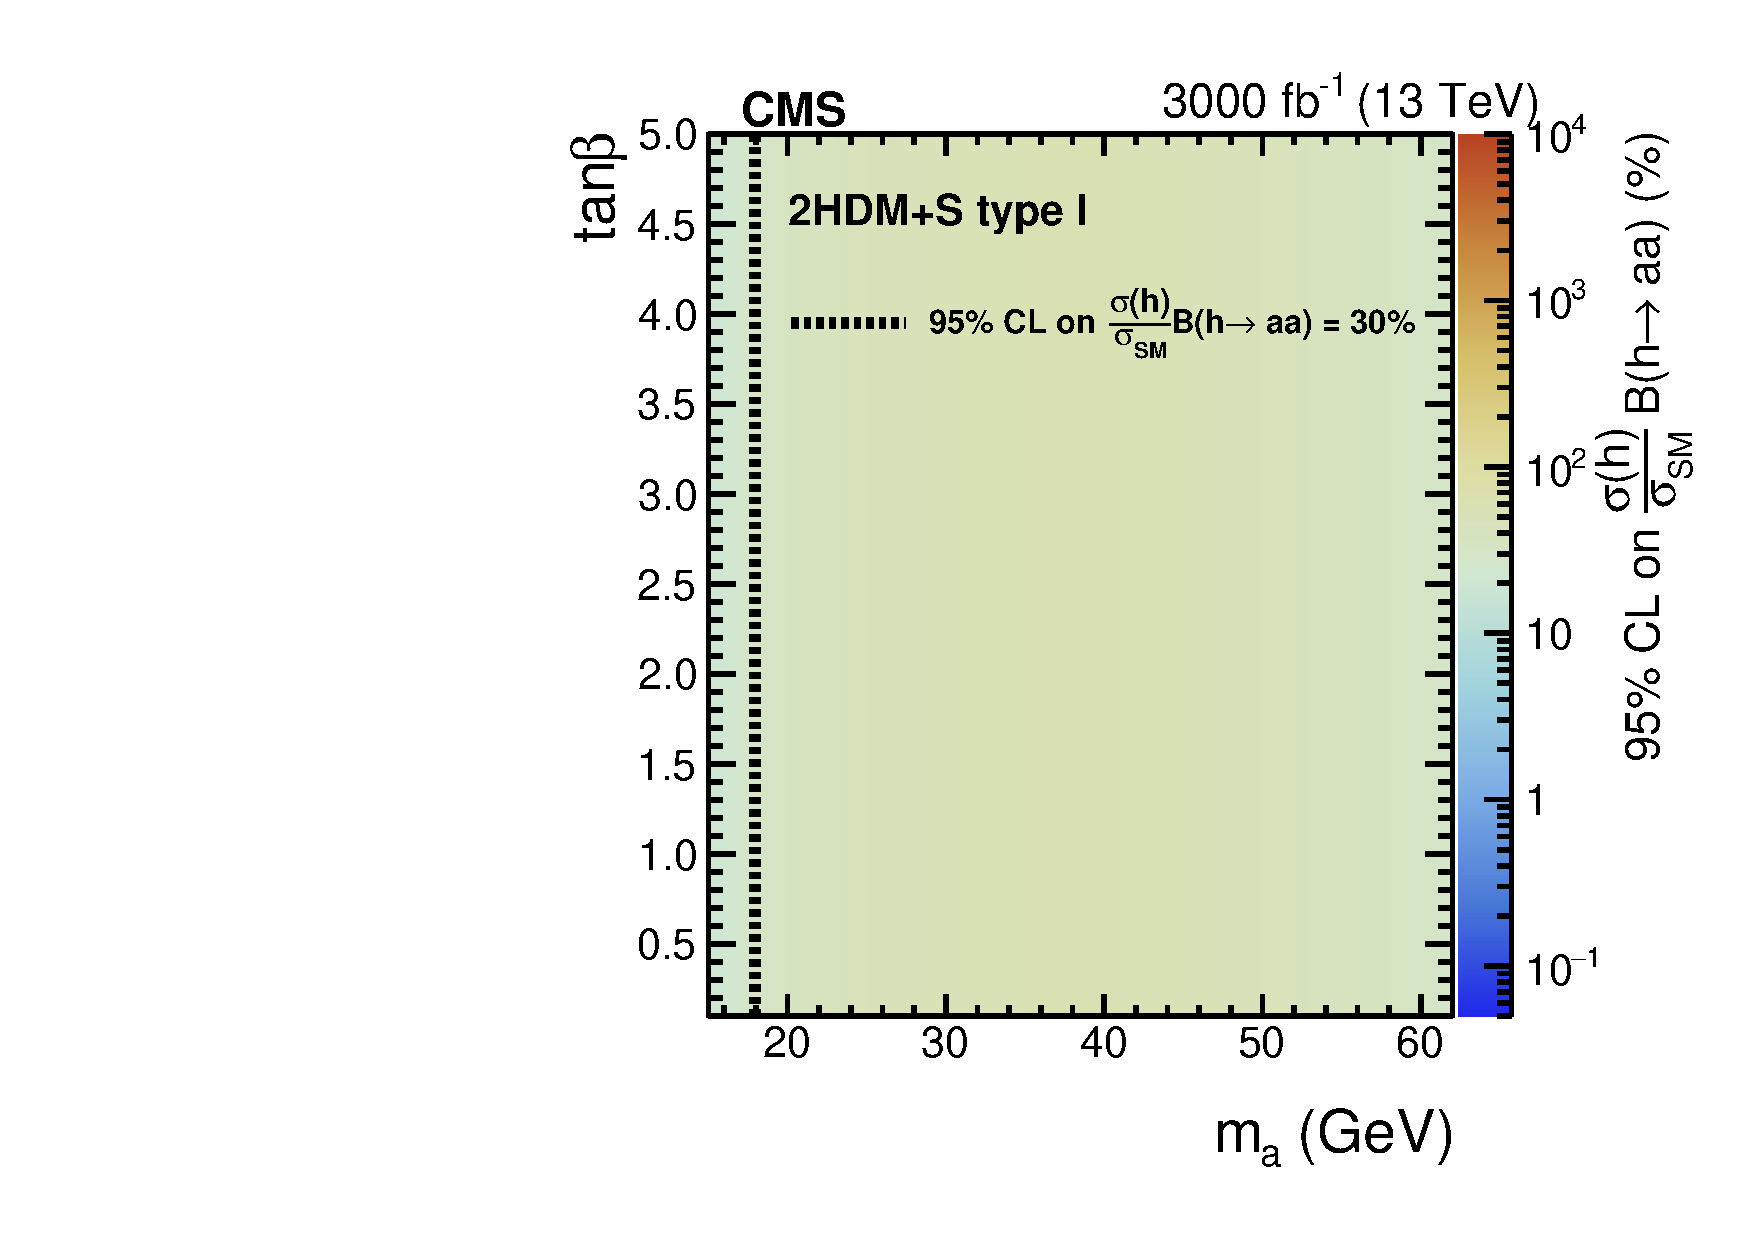
\includegraphics[width=0.49\textwidth]{\main/section9/plots/plot_BRaa_mmttProjection_Type1.pdf}
        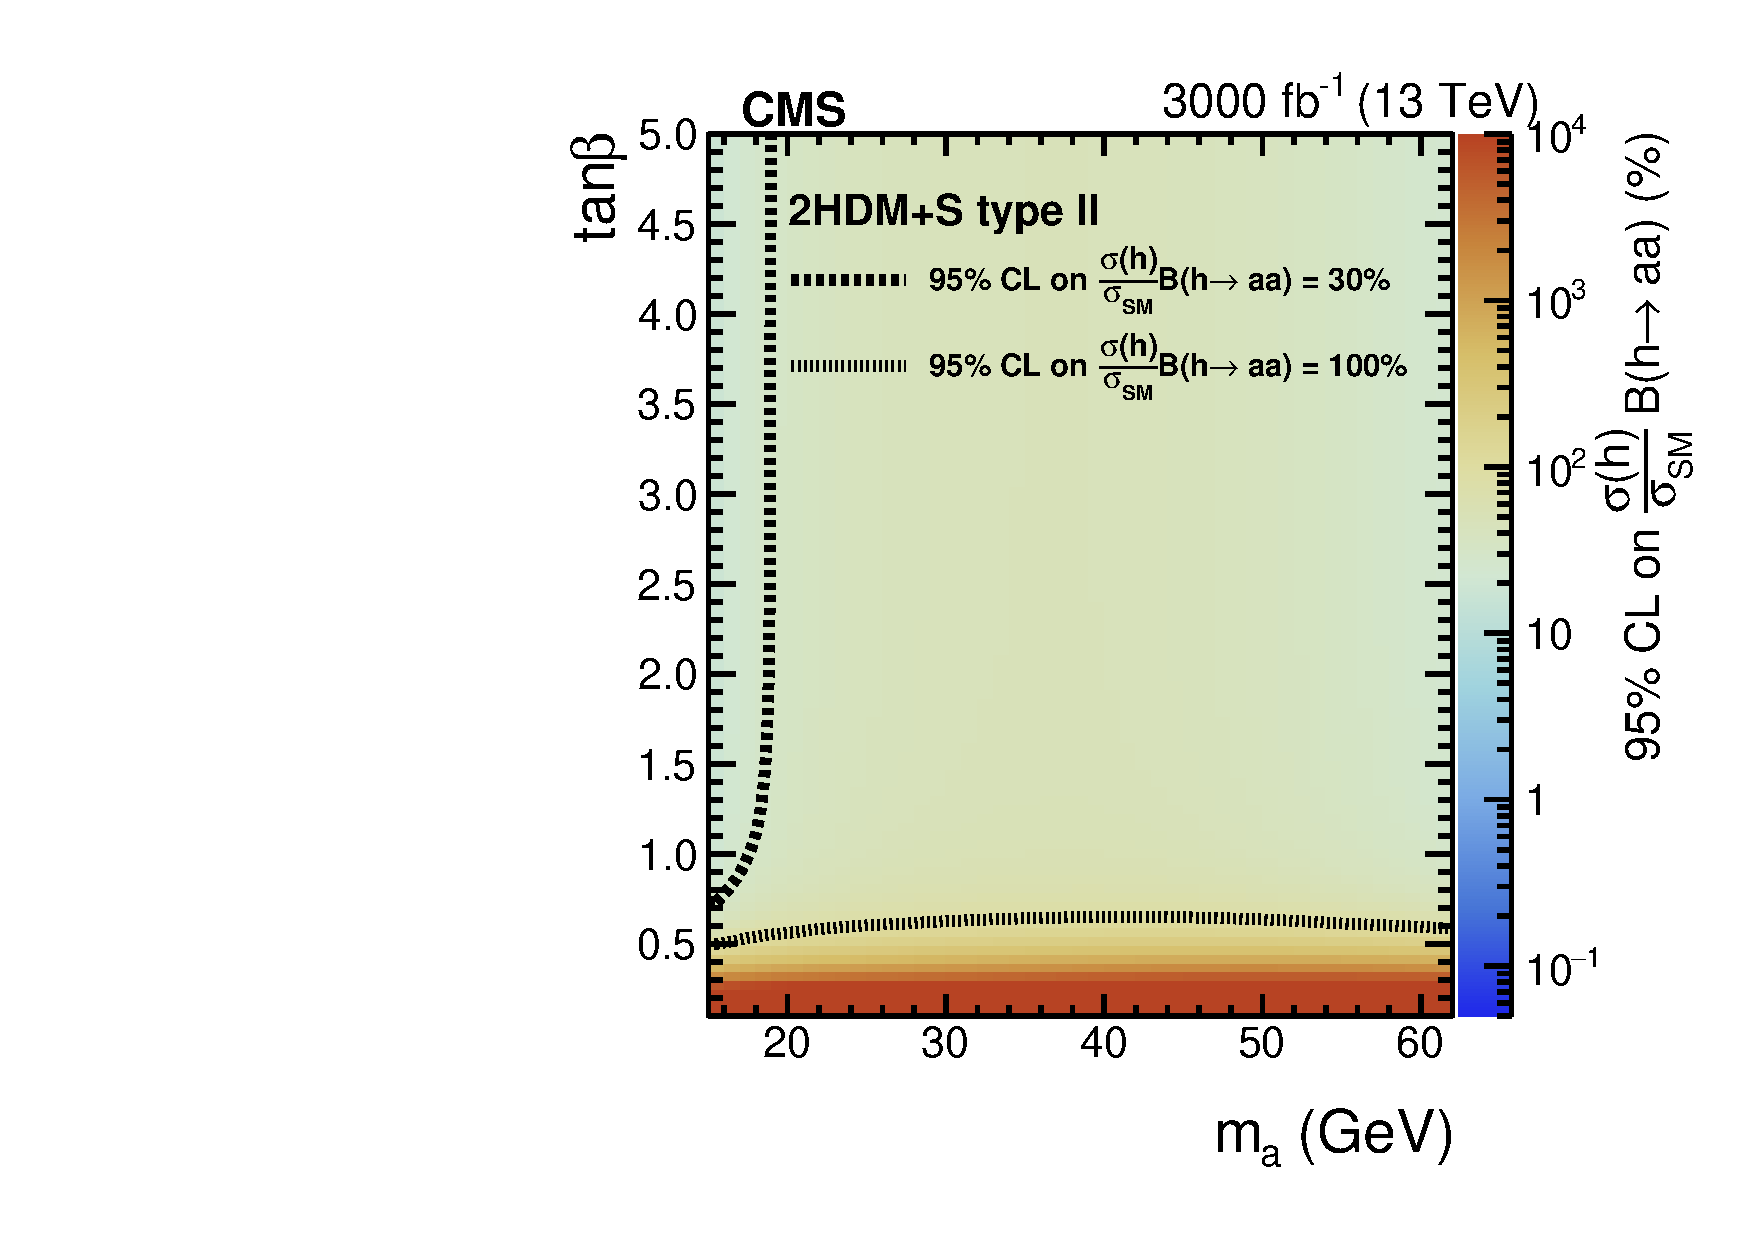
\includegraphics[width=0.49\textwidth]{\main/section9/plots/plot_BRaa_mmttProjection_Type2.pdf} \\
        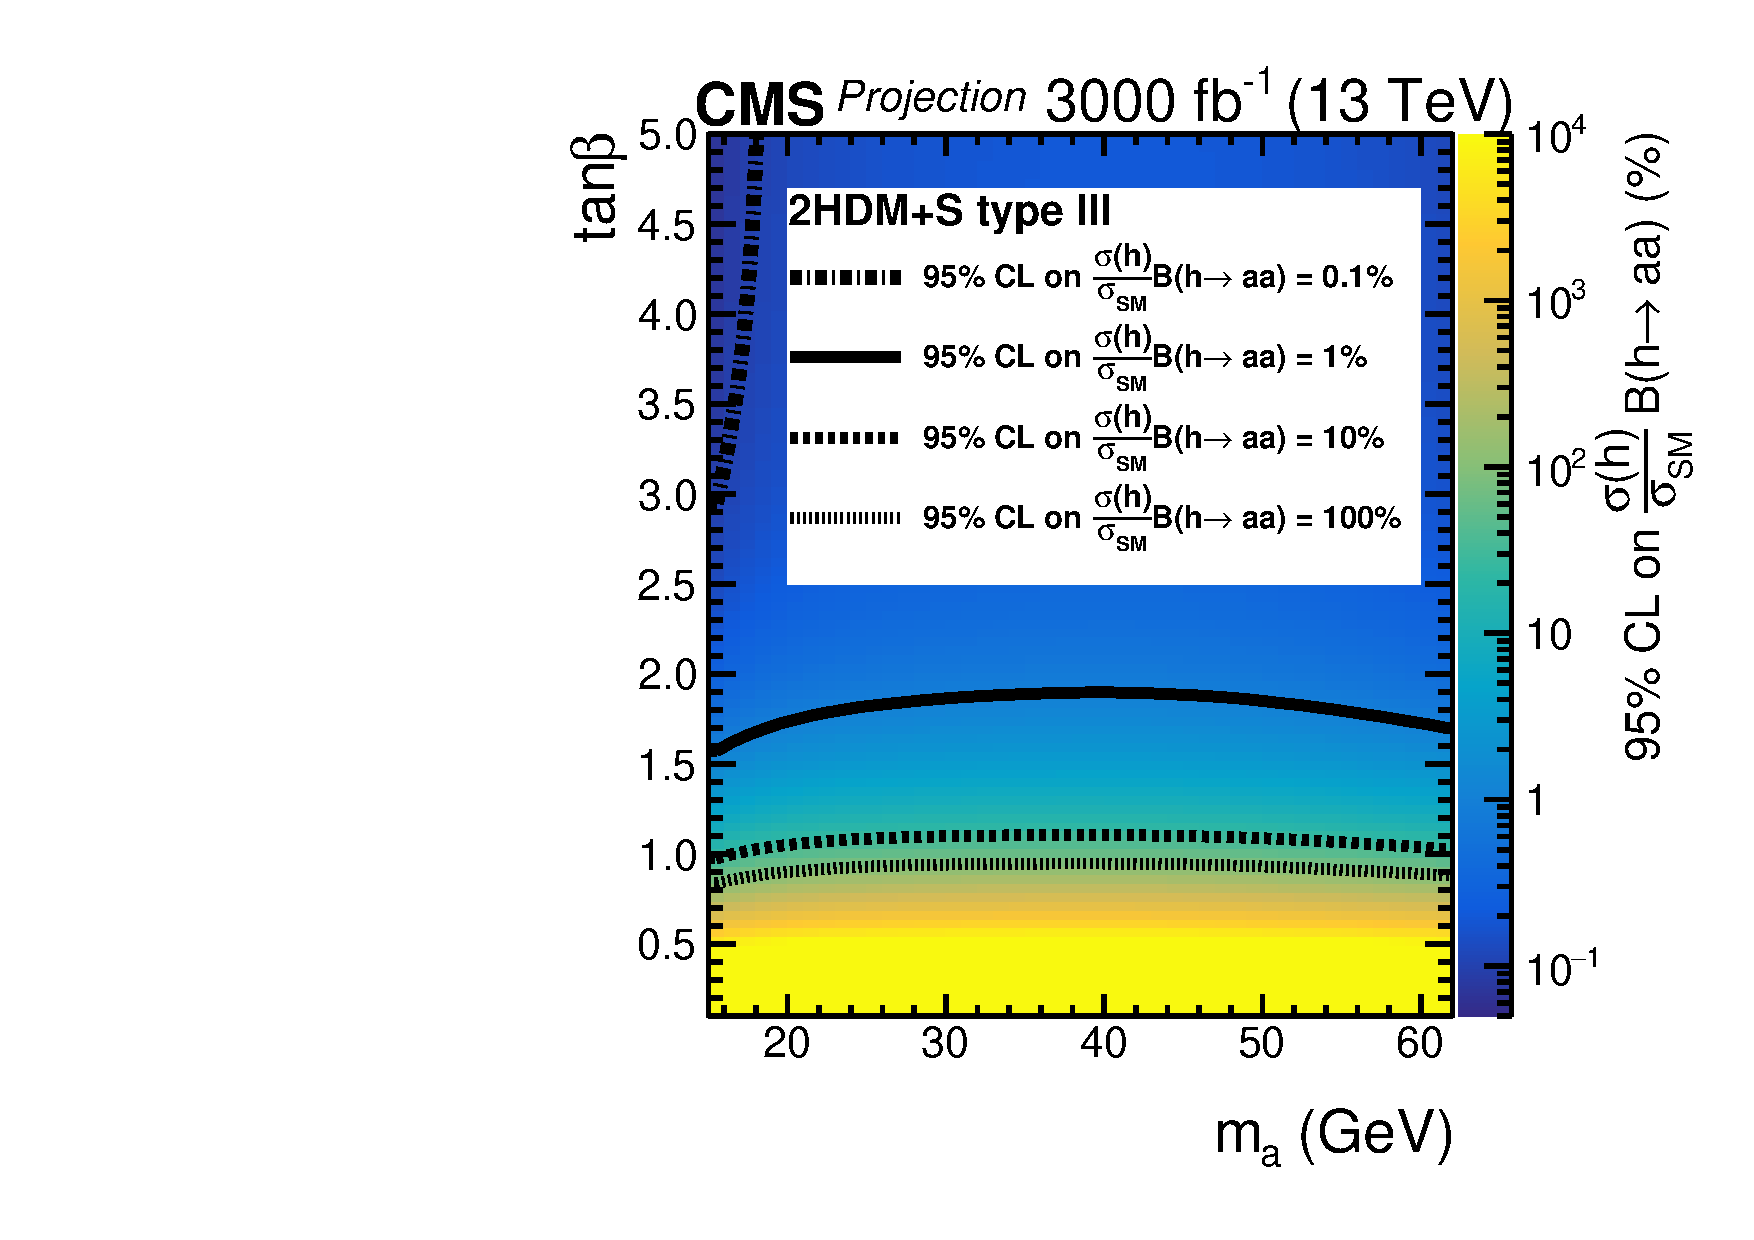
\includegraphics[width=0.49\textwidth]{\main/section9/plots/plot_BRaa_mmttProjection_Type3.pdf}
        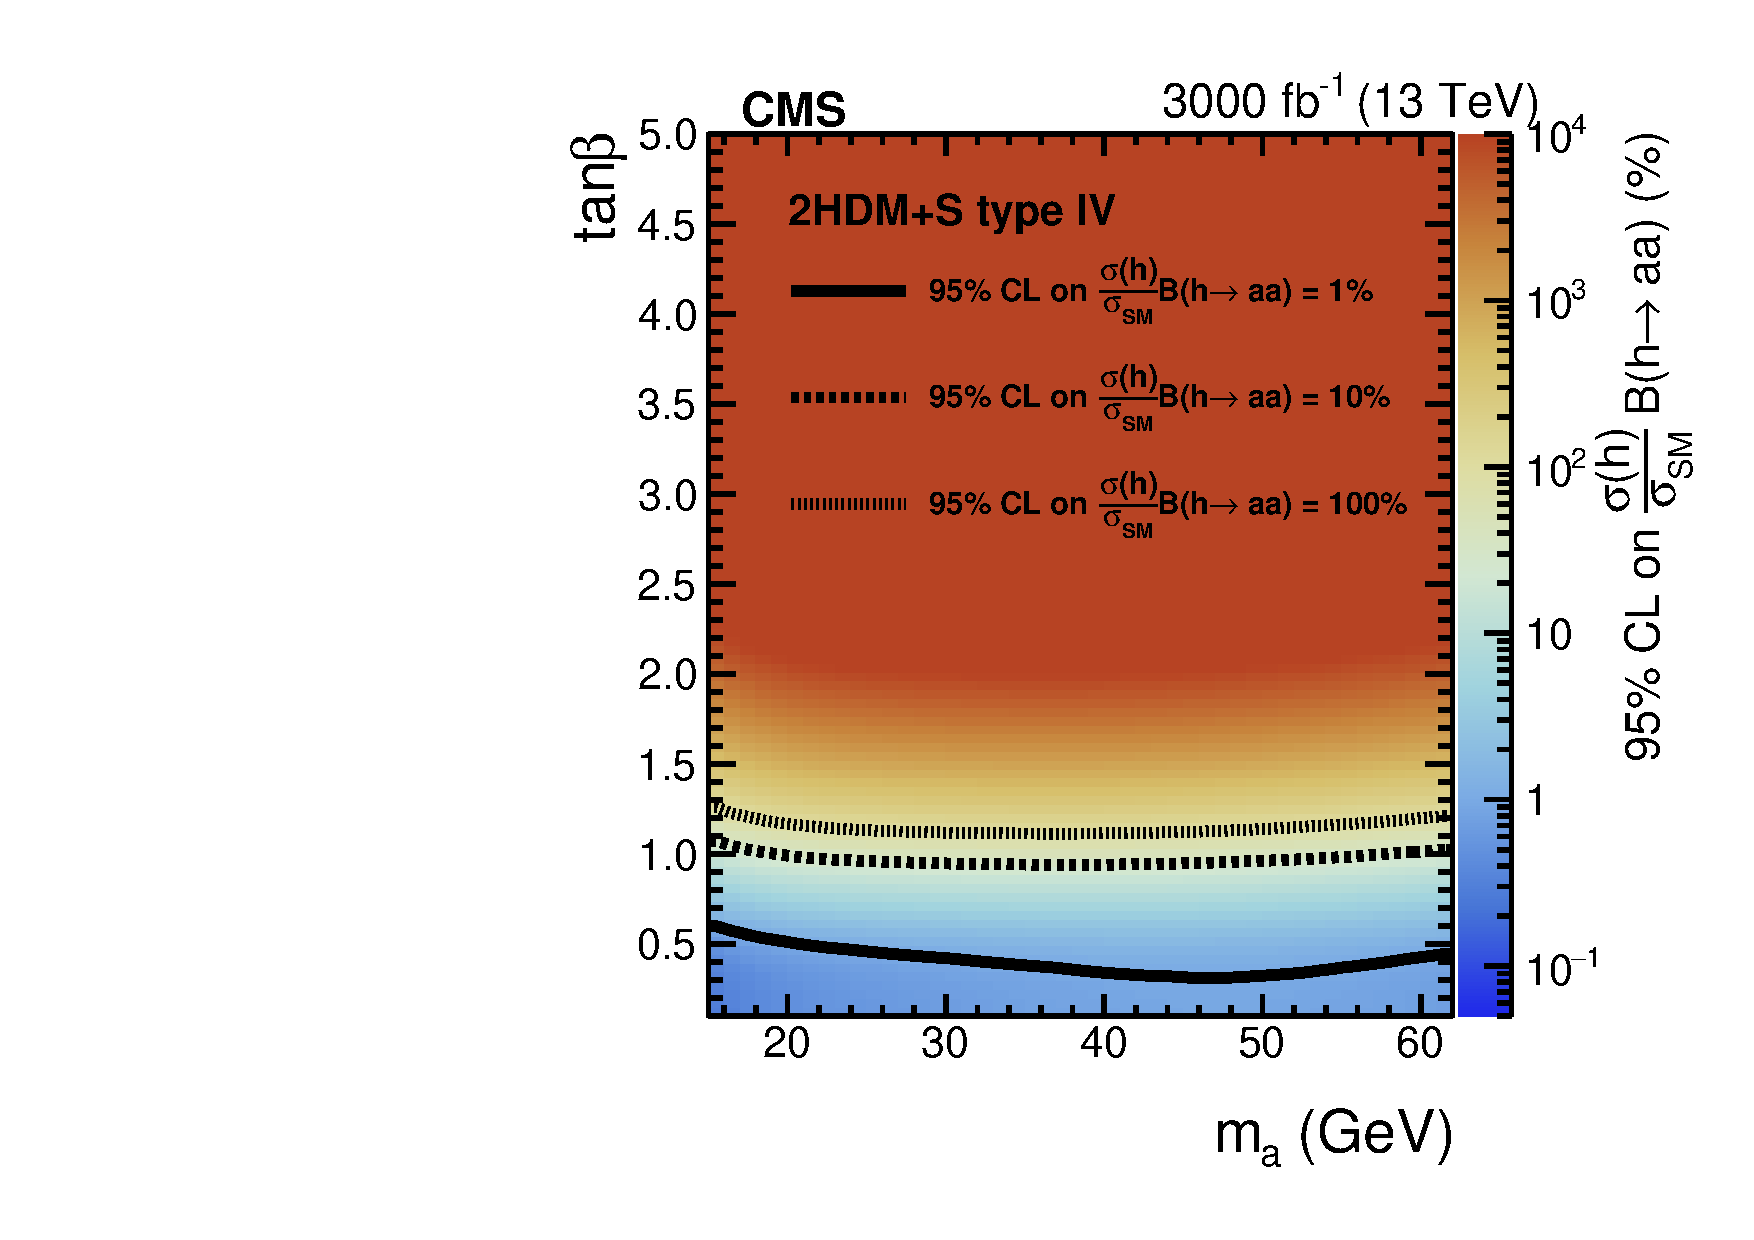
\includegraphics[width=0.49\textwidth]{\main/section9/plots/plot_BRaa_mmttProjection_Type4.pdf}
    \caption{Expected upper limits on $(\sigma(h)/\sigma_{\textrm{SM}})\mathcal{B}(h\to aa)$ for 3000\fbinv of data with YR18 systematic uncertainties for the $2\mu 2\tau$ final state in 2HDM+S type-1 (top left), type-2 (top right), type-3 (bottom left), and type-4 (bottom right).}
    \label{fig:summary_mmtt}
\end{figure*}


